\documentclass[conference, 10pt]{IEEEtran}
\usepackage{hyperref}
\usepackage{url}
\usepackage{latexsym}
\usepackage{graphicx}
\usepackage{amsmath}
\usepackage{amsthm}
\usepackage{amssymb}
\usepackage{amsfonts}
\usepackage{epsfig}
\usepackage{cite}
\usepackage{calc}
\usepackage{color}
\usepackage{subfigure}
\usepackage{algorithm}
\usepackage{algpseudocode}
%\usepackage{enumitem}
%\usepackage{lipsum}


\DeclareGraphicsExtensions{.jpg, .eps}
%\DeclareGraphicsRule{.jpg}{eps}{.jpg.bb}{`jpeg2ps -h -r 600 #1} 

\newtheorem{thm}{Theorem}
\newtheorem{cor}{Corollary}
\newtheorem{lem}{Lemma}
\newtheorem{prop}{Proposition}
\newtheorem{defn}{Definition}
\newtheorem{ex}{Example}
\newtheorem{remark}{Remark}

%\newcommand{\alglabel}[1]{\newcounter{#1}\setcounter{#1}{\value{ALC@line}}}
%\newcommand{\algref}[1]{\arabic{#1}}
\newcommand{\abs}[1]{\lvert #1 \rvert}
\newcommand{\flr}[1]{\lfloor #1 \rfloor}
\newcommand{\cel}[1]{\lceil #1 \rceil}
\newcommand{\mc}[1]{{\mathcal{#1}}}
\newcommand{\card}[1]{\abs{#1}}
\newcommand{\norm}[1]{{\|{#1}\|}}
\newcommand{\normsq}[1]{{\|{#1}\|}^2}
\newcommand{\ind}[1]{{\mathbb I}_{\{#1\}}}
\newcommand{\wedef}{\stackrel{\triangle}{=}}
\newcommand{\nth}[1]{{#1}^{\text{th}}}
\newcommand{\smfrac}[2]{{\textstyle{\frac{#1}{#2}}}}
\newcommand{\mybox}{\raisebox{3pt}{$\fbox{}$}}
\newcommand{\comm}[1]{{\bf COMMENT:} #1}
\newcommand{\mU}{{\mathcal{U}}}
\newcommand{\tr}{{\tilde{r}}}
\newcommand{\tX}{{\tilde{X}}}
\newcommand{\tL}{{\tilde{L}}}
\newcommand{\mM}{{\mathcal{M}}}
\newcommand{\mP}{{\mathcal{P}}}
\newcommand{\mI}{{\mathcal{I}}}
\newcommand{\mJ}{{\mathcal{J}}}
\newcommand{\mL}{{\mathcal{L}}}
\newcommand{\mO}{{\mathcal{O}}}
\newcommand{\bp}{{\mathbf{p}}}
\newcommand{\bb}{{\mathbf{b}}}
\newcommand{\bg}{{\mathbf{g}}}
\newcommand{\bz}{{\mathbf{z}}}
\newcommand{\bm}{{\mathbf{m}}}
\newcommand{\bK}{{\mathbf{K}}}
\newcommand{\mD}{{\mathcal{D}}}
\newcommand{\bA}{{\mathbf{A}}}
\newcommand{\ba}{{\mathbf{a}}}
\newcommand{\Ex}{{\mathbb{E}}}
\newcommand{\bPi}{{\boldsymbol{\Pi}}}

%\newcommand{\bpf}{\begin{proof}}
%\newcommand{\epf}{\end{proof}}
%\newcommand{\bdefn}{\begin{defn}}
%\newcommand{\edefn}{\end{defn}}
%\newcommand{\bprf}{{\em Proof: }}
%\newcommand{\bproof}{{\em Proof of }}
%\newcommand{\eproof}{\hfill $\Box$}
%\newcommand{\fix}{\marginpar{FIX}}
%\newcommand{\new}{\marginpar{NEW}}

%%%%%%%%%%%%%%%%%%%%%%%%%%%%%%%%%%%%%%%%%%%%%%%%%%%%%%%%%%%%%%%%%%%%%%%%%%%%%%%%%%%
\iffalse


- Motivation and Localization Problem

- Our approach

- Machine Learning Problem Statement

- Algorithm

- Extension to observation modeling

- Results

\fi

\title{Mobile Device Localization in 5G Wireless Networks}
% author names and affiliations
%\author{Paper Id: xxxx}
\author{\IEEEauthorblockN{Dandan Wang, Gurudutt Hosangadi, Pantelis Monogioudis, Anil Rao}
%\author{\IEEEauthorblockN{xxx, xxx, xxx,  xxx}
\IEEEauthorblockA{Nokia \\
Murray Hill, NJ, USA \\
\emph{\{dandan.wang, gurudutt.hosangadi, pantelis.monogioudis, anil.rao\}@nokia.com}}
%\emph{\{xxx, xxx, xxx, xxx\}@nokia.com}}
}


\begin{document}
\maketitle

%\setlist[itemize]{leftmargin=*}

\begin{abstract}

As wireless networks are evolving into 5G, tremendous data will be shared on the newly developed open source platforms. These data can be used
in developing new services. Among which, location information
of mobile devices are extremely useful. For example, the location information can be used to assist
wireless operators to trouble shoot the network performance. It can also be used to provide some location assisted service. However, some of these devices may be designed for
limited budget that do not have the capability of GPS. Furthermore, operators may not have access to the GPS information
on the mobile devices. In this paper, we propose a novel machine learning based approach to estimate the location of the mobile devices 
based on the measurement data that mobiles reported during every call and session. Our proposed algorithm utilizes the advanced features of 5G wireless network, such as the beam information.
Simulation shows that the proposed solution can achieve 10~m accuracy for mixed LoS and NLoS enviorment. And the proposed algorithm can also work even with only the information from one base station. 

\end{abstract}

%\let\labelindent\relax

\section{Introduction}


%Importance of measurements

Fueled with the emerging cloud technologies (cloud computing, cloud storage, etc), software defined network (SDN) together with 
network functions virtualization (NFV) is transforming the techonology, and business models in telcommunication industry.
Several open source platforms (ONAP, XRAN, etc) have emerged to provide a platform to collect data and share technologies among different 
vendors and operators. As the wireless network is now evolving into 5G, large amounts of data will be shared in these open source platform and thus create 
a lot of opportunity to provide better service using these data. The shared data can include a wide variety of measurements, such as the service throughput of the mobile 
device, the serving cell, the signal strength, etc. In ~\cite{Pantelis2016Localization}, a novel localization algorithm has been proposed to estimate 
the location when measurement reports are made in LTE systems. The paper shows that the medium accuracy of 20m can be achieved for outdoor mobibles. 
When celluar network evolves from 4G LTE to 5G, a lot of changes have been made to support lower latency and higher throughput. While multiple input multiple output (MIMO) has been extensively used in LTE, the most profound advancement of technology adopted in 5G
network is the utilization of a high number of (massive) MIMO antennas especially in the high band. With the use of massive MIMO, transmit power can be effectively beamformed and the mobile will report beam related metric to the base station. 
Therefore, the approach proposed in ~\cite{Pantelis2016Localization} for LTE can not be used directly for 5G network. In this paper, we propose a new localization algorithm to estimate the location of mobile devices utilizing the new reported metric introduced in 5G network.
 
%Our goal - loc and class
% As the open source platforms (such as ONAP, XRAN, etc) are still being developed,  it provides an opportunity to request different measurement 
% metrics. 
% The goal of this work are two folds: 1). identify the measurements unique to 5G network for localization.
% 2). estimate the latitude-longitude of the mobile using the measurement record
% generated in 5G network. 
%Our approach

In this paper, we design the localization algorithm combining the unique RF 
fingerprinting in 5G network and probablitistic path-tracking used for robot localization. The unique property of 5G network, such as the beam related 
information is used in this paper. The focus of this paper is on estimating location for outdoor mobiles. 
At a high level, our approach has two steps:

\begin{enumerate}
    \item Instead of viewing each NR UE measurement data (NUMD) record in isolation, for each mobile, we {\em stitch}
together NUMD records from that mobile over a ``session
duration"  and model it as a suitable Markovian time series. The problem now
reduces to identifying locations (states) of the entire path of
the mobile.

\item The above solution method assumes that the probabilities characterizing the
underlying Markovian structure can be learned. This is done by performing supervised learning using the beam information of 5G networks.
The training data for supervised learning may come from
drive test carried out by network providers once 5G is deployed commonly in the field. However, given that 5G network deployment is not available in the field during this study, we generate the drive training data and testing data from a 5G simulator.
	
\end{enumerate}

The details of the above two steps are provided in Section~\ref{sec:localalgo}.


Our main contribution in this paper is that we have proposed a new localization algorithm
appliable to 5G network. Based on our best knowledge, this is the first localization algorithm designed for 5G network. 


The rest of the paper is organized as follows. Section~\ref{sec:bg} provides some
background and introduces relevant terminologies. Section~\ref{sec:ps} presents
the problem setting and states the precise localization problem.
Section~\ref{sec:localalgo}
presents the main localization algorithm and Section~\ref{sec:channel-model} describes how to get the likehihood of the observation using machine learning approach. 
We present experimental validation in Section~\ref{sec:eval} and finally we conclude in
Section~\ref{sec:concl}.

%Contributions



\section{Relevant 5G Terminologies}
\label{sec:bg}
Though our techniques could apply to any future cellular system, we use $5$G New Radio (NR) 
terminologies for convenience. The terminologies~\cite{3gpp38series} relevant for our purpose are described below.

{\em UE (user equipment):} UE refers to the mobile end-device.

{\em Cell:} In $5$G networks, a cell refers to coverage footprint of a gNodeB transmitter. Since $5$G networks are expected operate in diverse spectrum bands, the cell coverage can vary from as low 100m to 5km. Typically, each cell is expected to cover an azimuth range of $120^\circ$ using sectorized antennas.

{\em gNodeB (gNB):} The gNB is the network element that interfaces with the UE and
hosts critical protocol layers like PHY, MAC, and Radio Link Control (RLC) etc. Each
gNB could have multiple transmission and reception points (TRP). Typical number number of TRPs is $3$ for full coverage around the gNB.

{\em Secondary Synchronization Reference Signal Received Power (SS-RSRP):} In $5$G networks, UEs make certain
measurements of received signal strength on the secondary synchronization (SS) signal for each nearby cell transmitter. SS-RSRP is
the total measured time-average received power at UE from the SS signals 
from a {\em given cell transmitter}. 

{\em Beam Indices:} In 5G-NR, there is the concept of a SS/PBCH block on the downink which comprises of a set of symbols ($4$) during which beamformed transmissions in a particular direction from gNB could take place. Each SS/PBCH block is identified by an index which the UE uses to report back measurements during a given SS/block. The beam indices we refer to in this paper correspond to the SS/PBCH block index and can have a range from $0$ to $63$ in standards. We use a grid of beams with upto $56$ possible directions in the performance evaluation section.  



% {\em RSSI and RSRQ} RSSI (Received Signal Strength Indicator) is the total measured
% received power at the UE over the entire band of operation from {\em all cell
% transmitters.} RSRQ of a given cell transmitter at a UE is RSSI scaled by average
% RSRP (of that cell) per reference symbol.

% We will need a figure to show the connection of 5G network to ONAP/xRAN, etc where the measured 
% data is stored.

\begin{figure}[t]
\begin{center}
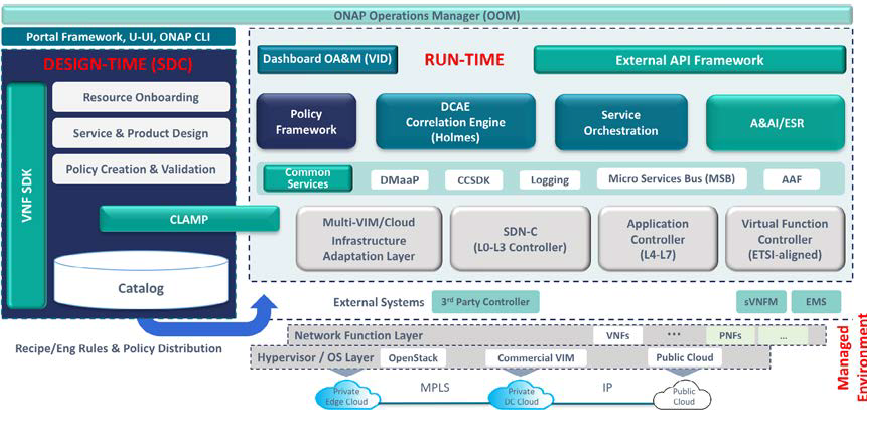
\includegraphics[height=3.0in,width=3.0in]{./ONAP-architecture.png}
\caption{\label{fig:onap_arch}
{\small ONAP architecture}}
\end{center}
\end{figure}



{\em ONAP} This stands for Open Nework Automation Platform and provides comprehensive platform for real time policy diven orchestration and automation of physcial and virtual network functions that will enable software, network,
IT and cloud providers and developers to rapidly create new services. Figure \ref{fig:onap_arch} shows the high level architecture. It is expected that in the context of $5$G networks and localization topic of this paper, ONAP would orchestrate the localization policy and associated cloud storage within the "Policy framework", "Data Collection, Analytics and Events (DCAE)" and "Service orchestration" components of the run-time module. 

{\em Measurement data collection architecture:} The NR UE measurement data (NUMD) collection process occurs primarily in the 5G network via the gNB and Mobility Management Entity (MME). The MME serves as the coordinator of the NUMD data.
After NUMD collection is turned on at the gNodeB, it collects the records and sends
the data to the MME. MME aggregates and temporarily saves NUMD from multiple
gNodeBs and sends it periodically (typically in minutes time-scale) to the data
center  where NUMD is saved and analyzed (for example, ONAP). Scalable storage of NUMD, which can easily
run into TB in a week per metropolitan, in the data center is an important design
problem and beyond the scope of this paper.


{\em Contents of NUMD:} NUMD record contains data related to signaling performance on
per UE, per bearer level for different procedures, user experience such as data
throughput and procedure duration, gNodeB internal UE related data such as MIMO
decision, SINR, buffer size, and normalized power headroom etc.  The information
present depends on procedure/event that led to the measurement record. For our
purpose, we are interested in RF information, and more specifically the SS-RSRP information contained in measurement records. 
%A NUMD record contains the following RF information:
%
%\begin{itemize}
%
%\item {\em RSRP:} Most NUMD contain RSRP of the serving cell that a UE is associated
%with. In addition, only when NUMD is generated due to an A3 or A4 event as described
%earlier in this section, it might also contain the RSRP of {\em one} neighboring
%cell (typically the strongest one).
%
%\item {\em beam indices:} NUMD also contains RSRQ of the serving cell. Note that once RSRP
%and RSRQ are known, the corresponding RSSI can be uniquely computed since RSRQ is
%defined as RSSI scaled by RSRP per reference symbol.
%
%\end{itemize}
%
%The important thing to note is that RSRP and RSRQ information is available from no
%more than two cells in an NUMD record.


%mobile measurement data, system, pcmd, data center, period



\section{Problem Statement} 
\label{sec:ps}

Consider in a 5G network, mobiles travel along a road represented by a graph $G_r=(V,E)$ where $V$
denotes graph nodes represented by a latitude-longitude tuple and $E$ denotes
valid direct path between two nodes. To estimate the location $V$ of this mobile, two types of data
are used in our proposed algorithm:

\begin{enumerate}

\item \textbf{Training data:} This is essentially geo-tagged data sent from
a set of locations in the road graph nodes $V$. The size of the training set is $n$, which include $n$ locations
$\{x_i\}_{i=1}^n$ and the corresponding SS-RSRP and beam indices at each location for each serving cell. Based on ~\cite{5GTF}, 
the mobile at each location can report up to four best beam indices and the corresponding SS-RSRPs.
We denote by $\{B^{j}_{i,k}\}_{i=1}^n$, the jth best beam indices sent from training location $x_i$ in cell $k$ and $\{R^j_{i,k}\}_{i=1}^n$ are the corresponding signal strength 
associated with those reported beam indices. Note
that, for a location $x_i$, the data $R^j_{i,k}$  and $B^j_{i,k}$ are only available
for a small subset of cells near location $x_i$. We will also denote the set of
training data by $\mathcal{D}_{tr}$.

\item \textbf{NUMD data or observed data:} This data is not geo-tagged but comes
with time stamp. Precisely, for every mobile, we are given time instants
$t_i, i=1,2,\hdots,T$ for each $t_i$ we are also given SS-RSRP
$\{{\tilde{R}}^j_k(t_i)\}_{j=1}^4$ and beam indices ${\{\tilde{B}}^j_k(t_i)\}_{j=1}^4$ where $k\in K(t_i)$; $K(t_i)$ denotes the set of cells reported by
the mobile at time~$t$. Typically $\card{K(t_i)}$ takes value one or two.
Though we have NUMD for each mobile-$m$, we drop the dependence of $m$
on $R_k(t)$ and $K(t)$ as we are essentially performing the same algorithm
for each mobile separately. The locations of mobiles $\tilde{x}(t_i)$ at different
times $t_i$ are unknown.
	
\end{enumerate} 

Thus the problem can be stated as follows:

{\bf Problem of localization in 5G network}: 
We are given training data consisting
of locations $\{x_i\}_{i=1}^n$ and the associated SS-RSRPs  $\{R^j_{i,k}\}_{i=1}^n$ and beam indices $\{B^j_{i,k}\}_{i=1}^n$ of
cell-$k$ at location $x_i$. Assume that the locations
are drawn from locations in a road network given by $G_r=(V,E)$. Thus, the problem is to estimate the unknown location of the mobiles when mobiles report a sequence of measurements
${\tilde{R}}^j_k(t_i)$ and ${\tilde{B}}^j_k(t_i)$ where $i=1,2,\hdots,L,\ k\in K(t_i), j=1, 2, 3, 4$. $L$ is the length of the sequence of the measurement reports.
Note that, in the algorithm illustration in this paper, we only focus on SS-RSRP and beam indices. However, in the field, there may be other measurement reports that 
can be used to help to improve the localization accuary. For example, timing alignment, etc. These addtional measurement reports can be easily incorporated into our proposed algorithm.

\section{Localization Algorithms}
\label{sec:localalgo}

The framework we use for tackling the localization problem is hidden markov model (HMM) as illustrated 
in Figure~\ref{fig:hmm_particle}. The hidden states in HMM in our case are the locations and the velocity. 
The observations corresponding to each hidden state are the reported measurement reports, such as SS-RSRP and the beam indices.
The system moves from one hidden state to another hidden state with some underlying mobility model. 
The goal is to infer the hidden state from the observations based on
prior knowledge about the transition probabilities between hidden states and
observations in the states. We assume that the mobile updates its speed according to Gauss-Markov Mobility Model ~\cite{Camp2002}.

\begin{align}
S_t = \alpha S_{t-1}+(1-\alpha)\bar{S}+\sqrt{(1-\alpha^2)}S_{x_{t-1}}
\label{eqn:speed}
\end{align}
\begin{align}
d_t = \alpha d_{t-1}+(1-\alpha)\bar{d}+\sqrt{(1-\alpha^2)}d_{x_{t-1}}
\label{eqn:speed}
\end{align}

 where $S_t$ and $d_t$ are the new speed and direction of the mobile at time interval t. $S_{x_{t-1}}$ and $d_{x_{t-1}}$
 are random variables from a Gaussian distribution with mean $\bar{S}$ and $\bar{d}$.
 
 At each time interval the next location is calculated based on the current location, speed, and direction of movement.
Specifically, at time interval t, a mobile's position is given by the equations.

\begin{align}
	l_t = l_{t-1} +S_{t-1}cos(d_{t-1})*\Delta t
\label{eqn:mobilitymodelx}
\end{align}
\begin{align}
h_t = h_{t-1} +S_{t-1}sin(d_{t-1})*\Delta t
\label{eqn:mobilitymodely}
\end{align}

where ($l_t$,$h_t$) and ($l_{t-1}$,$h_{t-1}$) are the latitude and longitude coordinates of the mobile’s position 
at time intervals $t$ and $t-1$, respectively. $\Delta t$ is the duration of the time interval.

However, it is difficlut to obtain analytic solutions for HMM and particle filter has been widely used to provide approximate solutions to these intractable inference problems~\cite{doucet2009tutorial}~\cite{ThrunParticleFilter}.
We also use particle filter approach in this paper. 

In the highlevel, the proposed localization algorithm, namely $5GLocalizeAlgo$, is stated as follows:
\begin{itemize}
	\item We first initialize a set of $N$ particles based on some priori distribution, for example, the coverage map of a base station.
	Here, particles are the samples of the possibles locations. 
	\item Each particle has its corresponding weights or likelihoods, which represents the likelihood of achieving the observations at each given particle (i.e., location in this case). This weight/likelihood is obtained using machine learning algorithm as illustrated in Section ~\ref{sec:channel-model}.
	\item Particles move from one state to another state based 
	on the state transition model given in equations (\ref{eqn:mobilitymodelx}) and (\ref{eqn:mobilitymodely}).
	\item In the end, the sequence of the particles which have the largest likelihood are the estimated locations. 
	\item The pseudocode is presented in Algorithm \ref{alg:LocalizeUEpf}. The inpputs are training data $D_{tr}$, the graph $G_r$ and the threashold $N_{th}$ used in resampling particle filter~\cite{ThrunParticleFilter}.
\end{itemize}

\begin{figure}[t]
	\begin{center}
	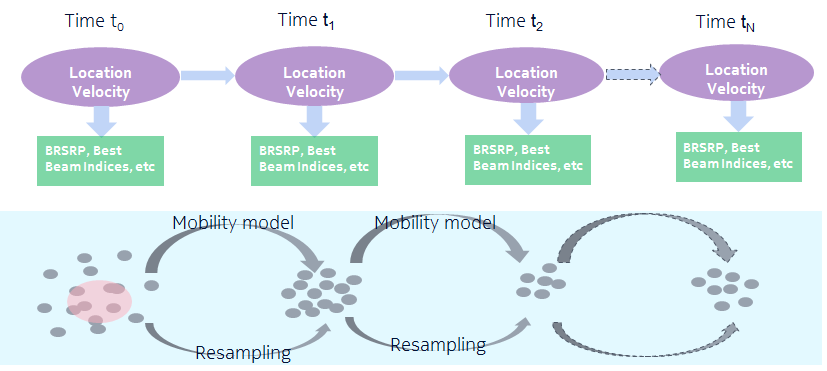
\includegraphics[height=3in,width=2.8in]{./HMM_ParticleFilter_Illustration.png}
	\caption{\label{fig:hmm_particle}
	{\small Hidden Markov Model and Particle filter}}
	\end{center}
	\end{figure}

\begin{algorithm}
\caption{$5GLocalizeAlgo(\mathcal{D}_{tr},G,N_{th})$}
\label{alg:LocalizeUEpf}
\begin{algorithmic}[1]
\State Offline inference based on training data $\mathcal{D}_{tr}$ to get the imortance weight associated with each particle. This does not need real time processing.
\State Sample $N$ particles $\mathcal{P}_j = \{\hat{x}_1^{(j)},\hat{v}_1^{(j)}\},$ $j=1,\hdots , N$ 
from prior distribution $p(\tilde{x}_1, \tilde{v}_1|G)$ 

\State Initialize importance weights $\hat{w}_1^{(n)} \gets p(\{\tilde{R}^j_1\}_{j=1}^4,\{\tilde{B}^j_1\}_{j=1}^4|\hat{x}_1^{(n)}),$ $n=1,\hdots , N$

\State Normalize $w_1^{(n)} \gets \hat{w}_1^{(n)}/\sum_{l=1}^N \hat{w}_1^{(l)},$ $n=1,\hdots , N$

\For{$i = 2$ to $L$}
	\For{$n=1$ to $N$}
		\State Sample $\hat{x}_i^{(n)}$ from $\hat{x}_{i-1}^{(n)}$ based on state transition model in equations (\ref{eqn:mobilitymodelx}) and (\ref{eqn:mobilitymodely}).
		\State Update weight $\hat{w}_i^{(n)} \gets \hat{w}_{i-1}^{(n)} \times p(\{\tilde{R}^j_i\}_{j=1}^4, \{\tilde{B}^j_i\}_{j=1}^4|\hat{x}_{i}^{(n)})$ 
	\EndFor
	\State Normalize $w_i^{(n)} \gets \frac{\hat{w}_i^{(n)}}{\sum_{l=1}^N \hat{w}_i^{(l)}}$
	\State $\hat{N}_{eff} \gets \frac{1}{\sum_{l=1}^N (w_{i}^{(l)})^2}$
	\If{$\hat{N}_{eff} < N_{th}$, $i<L$ (excluding the last point in the sequence), resampling condition satisfied}
		\State Sample $N$ particles with replacement from current particle set $\{\mathcal{P}_j\}_{j=1}^N$ with probabilities $\{\hat{w}_i^{(j)}\}_{j=1}^N.$ Update particle set with the new sampled set
		\State $w_i^{(n)} \gets \frac{1}{N}$ for $n=1,\hdots , N$
	\EndIf
\EndFor
\State $n^* = \arg \max_{n = 1 , \hdots, N} w_L^{(n)}$

\State Output location estimate $\{\hat{x}_i^{(n^*)}\}_{i=1}^L$ 
\State Output distribution \\
$p(\{\hat{x}^{(n)}\}_{i=1}^L|\{\tilde{R}^{1,2,3,4}_i\}_{i=1}^L,\{\tilde{B}^{1,2,3,4}_i\}_{i=1}^L,G) = w_L^{(j)}$ for $n=1$ to $N$
\end{algorithmic}
\end{algorithm}  


\section{Observation modeling using machine learning}
\label{sec:channel-model}
As mentioned in the above section, one of the important inference of HMM is the likelihood of achieving the observation at the given paritcle. In this section, we discuss how to infer the likehihood using machine learning approach. 
\subsection{Inference on likelihood of beam indices}
\label{sec:prob-classification}
As part of the observations of HMM model, UE reports up to four observed best beam indices. The probability
distribution (also called the likelihood function) of a particular observed beam index such as its $j$-th ($j=1, 2, 3, 4$) best reported beam indices
at a given location is denoted by
$p(\tilde{B}^j_i|\hat{x}_{i})$. In our approach, these probabilities
can be learnt from the drive test data using machine learning classification algorithms.

Following are the steps to obtain the inference:

\begin{enumerate}

\item For each location in the training set, we
take the corresponding reported beam indices. Then, pre-processing is done to separate the data based on the cell ID and whether it is best beam index, or second/third/fourth best beam index.

\item For each cell, we obtain the likelihood of a certain class (i.e., beam index) using classifier where the latitude and the longitude are 
taken as features of the model and the likelihood of the beam indices is the output. Different cells are trained using their own data sets. Even for the same
cell, each best beam index will be trained seperately, meaning, the best beam index, the second best beam index, the third best beam index and the fourth best beam index each has their own trained model.
Each such classifier is trained using the data aggregated in the previous step.

\item There are different machine learning classifiers in the literature. Considering the strong spatial correlation of the beam index, and also we will need to get the probability of class, random forest classifier is considered as a good choice. 
In this paper, we use the random forest classifier in the machine learning library (sklearn) to predict the probability of 
reporting a specific beam indices. The function $predict\_proba(X)$ can be used to get the probability of class $X$. Note that different classifiers were tested in the study and we found that
neruon network and random forest provide similar performance. However, given more intuitive illustration of random forest, we decide to use random forest classifier.
\end{enumerate}
\subsection{Inference on likelihood of SS-RSRP}
\label{sec:prob-reg}
Similar to beam indices, the SS-RSRP reported at different states
is also part of the observations of HMM model. The probability
distribution (also called the likelihood function) of an observed SS-RSRP on a location is denoted by
$p(\tilde{R}_i|\hat{x}_{i})$. In our approach, these probabilities
can be learnt from the training data using machine learning regression algorithms. 

Following is the steps to obtain the inference for SS-RSRP:

\begin{enumerate}
\item For each location, each base station and each reported set of beam indices, we
take the empirical mean and variance of all corresponding drive test data SS-RSRP. Note that for each location, there may be multiple reported SS-RSRP as SS-RSRP varies when measured at different time.

\item Similar with the inference on beam index, random forest regressor is a good choice here. For each cell and each beam indices, model the spatial variation of SS-RSRP-statistics (i.e., mean and
standard deviation) using {\em Random Forest} where the latitude and the longitude are 
taken as features of the model and the SS-RSRP-statistic  of the cell is the output. Each such {\em
Random Forest} is trained using data aggregated in previous step. Also,
computed is the mean square error (or {\em cross validation error})
for each random forest. 

\item Denote by $RndFrst_m(x,b,c)$ ($RndFrst_s(x,b,c)$) the random forest predictor of
mean (standard deviation) of SS-RSRP for cell-$c$, beam-$b$
at location $x$. Let $(\sigma_{RF}(b,c))^2$ be the corresponding
mean square error of the predictor. Then we model
\begin{align}
p(\tilde{R}^j_i|\hat{x}_{i}, \tilde{B}^j_i) =
\mathcal{N}(RndFrst_m(\hat{x}_{i},b,c), \sigma_c^2(\hat{x}_i))\ ,
\label{eqn:rndfrst}
\end{align}
where $$\sigma_c^2(x) = RndFrst_s(x,b,c) + \sigma_{RF}^2(b,c)\,$$ 
and the serving cell-$c$ can be obtained from the NUMD record. $\mathcal{N}$ represents the Gaussian distribution.
In general, we
can choose any spatial regressor instead of random forest. However, choosing
random forest makes the model robust to cell propogation properties and to the
fact that the coverage area of the cell could be disjoint.
\end{enumerate}

Note that in in 5G network, with the existence of beams, the regression algorithn is now implemented per cell and per beam index.

\subsection{Inference on the likelihood of combined observations}
\label{sec:prob-combined}
The likelihood of seeing all the observations, $\{\tilde{R^j_i}\}_{j=1}^4$ and $\{\tilde{B^j_i}\}_{j=1}^4$ at a given location $\hat{x}_{i}$ is as follows:

\begin{equation} 
\begin{split}
	p(\tilde{R}^1_i, \tilde{R}^2_i, \tilde{R}^3_i,\tilde{R}^4_i, \tilde{B}^1_i, \tilde{B}^2_i, \tilde{B}^3_i, \tilde{B}^4_i|\hat{x}_{i})
	\\
	=\prod_{j=1}^4 p(\tilde{R}^j_i|\hat{x}_{i}, \tilde{B}^j_i)p(\tilde{B}^j_i|\hat{x}_{i}),
\end{split}
\label{eqn:combined}
\end{equation}
where $p(\tilde{R}^j_i|\hat{x}_{i}, \tilde{B}^j_i)$ and $p(\tilde{B}^j_i|\hat{x}_{i})$ are obtained in the section \ref{sec:prob-classification} and \ref{sec:prob-reg}.
%%%%%%%%%%%%%%%%%%%%%%%%%%%%%%%%%%%%%%%%%%%%%%%%%%%%%%%%%%%%%%%%%%%%%%%%%%%%%%%%%%%%%%%%%%
%\iffalse

% \section{Extension: Joint Localization and Channel Modling}
% \label{sec:extensionalgo}
% In this section we describe our main algorithm for joint observation modelling and UE
% localization. The Joint Observation Modeling and Localization (JOML) algorithm takes
% as input the labeled and unlabeled datasets $\mathcal{D}_1,\mathcal{D}_2,$ the
% graph $G$ and a parameter $N_{em}$ specifying the number of
% expectation-maximization (EM) iterations to be performed. It outputs the UE
% location estimates $\{\hat{x}_i\}_{i=1}^m$ and the observation model $\mathcal{C}$
% in the region of interest. The main idea is to use expectation-maximization
% procedure to iteratively improve the estimates of both the observation model
% $\mathcal{C}$ and the location estimates $\{\hat{x}_i\}_{i=1}^m.$ The basic EM
% algorithm improves the channel in each iteration from the previous according to
% the following equation.

% \begin{equation}
% \mathcal{C}^{t+1} = \arg \max_{\mathcal{C}} E_{\{\hat{x}_i\}_{i=1}^m |\mathcal{D}_1,\mathcal{D}_2,\mathcal{C}^t} \log  P(\mathcal{D}_1,\mathcal{D}_2,\{\hat{x}_i\}_{i=1}^m|\mathcal{C}) \label{eq:EM}
% \end{equation}

% The high level pseudo-code of the algorithm is shown in Algorithm \ref{alg:joint_ch_model_loc}.  

%\begin{algorithm}
%\caption{$JCML(\mathcal{D}_1, \mathcal{D}_2, G, L_{th})$}
%\label{alg:joint_ch_model_loc}
%\begin{algorithmic}[1]
%\State $\mathcal{D} \gets \mathcal{D}_1$
%\State $\mathcal{C} \gets ChannelModel(\mathcal{D})$
%\For{$i=1$ to $m$}
%	\State $\{\hat{x}_j\}_{j=1}^i \gets %LocalizeUE(\{\tilde{R}_j,T_j\}_{j=1}^i,\mathcal{C},G)$ \label{step:localize}
%	\State $\mathcal{D} \gets \mathcal{D}_1 \cup %\{\tilde{R}_j,\hat{x}_j\}_{j=1}^i$
%	\State $\mathcal{C} \gets ChannelModel(\mathcal{D})$
%\EndFor
%\State Output $\{\hat{x}_i\}_{i=1}^m, \mathcal{C}$
%\end{algorithmic}
%\end{algorithm}  

% \begin{algorithm}
% \caption{$JOML(\mathcal{D}_1, \mathcal{D}_2, G, N_{em})$}
% \label{alg:joint_ch_model_loc}
% \begin{algorithmic}[1]
% \State $\mathcal{C} \gets Observation Model(\mathcal{D}_1)$ based on section ~\ref{sec:channel-model}.
% \For{$j = 1$ to $N_{em}$}
% 	\State $\{\hat{x}_i\}_{i=1}^m, p(\{\hat{x}_i,\tilde{R}^j_i,\tilde{B}^j_i\}_{i=1}^m|\mathcal{C},G) \gets 5GLocalizeUE(\mathcal{D}_2,\mathcal{C},G)$ as in Algorithm \ref{alg:LocalizeUEpf}. \label{step:localize}
% 	\State $\mathcal{D} \gets \mathcal{D}_1 \cup \{\tilde{R}_i,\hat{x}_i\}_{i=1}^m$ \label{line:em_approx}
% 	\State $\mathcal{C} \gets Observation Model(\mathcal{D})$ based on section ~\ref{sec:channel-model}.
% \EndFor
% \State Output $\{\hat{x}_i\}_{i=1}^m = \arg \max_{\{\hat{x}_i\}_{i=1}^m} p(\{\hat{x}_i,\tilde{R}_i, \tilde{R}_i\}_{i=1}^m,|\mathcal{C},G)$
% \State Output $\mathcal{C}$
% \end{algorithmic}
% \end{algorithm}  

%  \textbf{[QUESTION: I see some inconsistency in the Algorithm 2 description. It is using Algorithm 1. However, Algorithm 1 is taking as input dataset, graph G and ${N_th}?$. While here it is taking as input dataset, C (a function) and G]} 

% Note that in line \ref{line:em_approx} $\{\hat{x}_i\}_{i=1}^m$ can be the mode
% or samples from the distribution
% $p(\{\hat{x}_i,\tilde{R}^j_i, \tilde{B}^j_i\}_{i=1}^m,|\mathcal{C},G)$ as a stochastic
% approximation for the EM algorithm. The JOML algorithm uses two main
% subroutines. The first subroutine $ObservationModel$ computes the likelihood function
% $\mathcal{C}$ from the labeled dataset $\mathcal{D}.$ $\mathcal{C}$ can be
% viewed as a function which can output the distribution of SS-RSRP and beam indices from any base
% station $k$ to any UE location $x \in V.$ The second subroutine $5GLocalizeUE$
% use the observation model function $\mathcal{C},$ the NUMD data
% $\{\tilde{R}_i,T_i\}$ and the graph $G$ to come up with location estimates of
% the UE $\{\hat{x}_i\}_{i=1}^m$ and its corresponding distribution as illustrated in section ~\ref{sec:localalgo}. Each time a
% location estimate is computed it is used with the corresponding record
% $\tilde{R}^j_i$, $\tilde{B}^j_i$ and the dataset $\mathcal{D}_1$ to further improve the channel
% model \textbf{[QUESTION: why are we calling this a channel model? Are we predicting the channel? Are we not only predicting SS-RSRP and beam indices?] } using an expectation-maximization procedure. Therefore in the next
% iteration we can obtain a better location estimate. 

%\fi
%%%%%%%%%%%%%%%%%%%%%%%%%%%%%%%%%%%%%%%%%%%%%%%%%%%%%%%%%%%%%%%%%%%%%%%%%%%%%%%%%%%%

\section{Evaluation}
\label{sec:eval}
In this section, we present evaluation results of our proposed algorithm. 
\subsection{Methodology}
In this paper, we focus on one isolated cell in 5G network, where the measurement report
only has the information of the serving cell. In the field, when we have multiple cells, the additional
information on the measurement report from neighboring cells can be easily incorporated into the proposed algorithm to improve the 
localization accuary. This could include information such as RSRQ and RSSI. As there is no commercial deployed 5G network yet, we dont have the drive test data from the field.
Instead, we use our 5G system simulator to generate both training data and test data.

The 5G system that we use in this evaluation is operating at mmwave band, and the cell ISD is 200m. The testing data points are illustrated in 
Figure ~\ref{fig:training}, which has 1000 data points. Instead of diving the training data into training and validation, we use the gridsearch and cross validation functionaility in 
sklearn ~\cite{sklearn} to avoid the overfitting since we have limited number of training data.

\begin{figure}[t]
	\begin{center}
	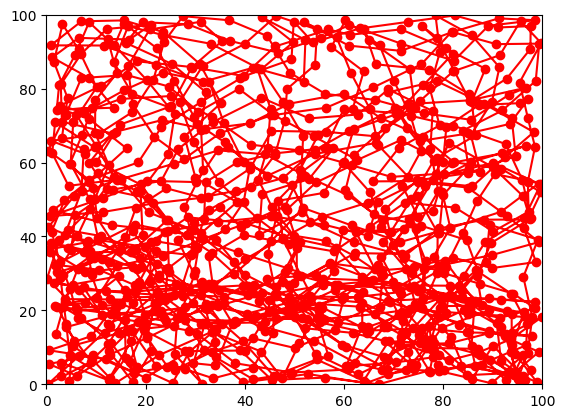
\includegraphics[height=2.4in,width=3.2in]{./GM_training.png}
	\caption{\label{fig:training}
	{\small Training data points}}
	\end{center}
	\end{figure}		

\subsection{Localization Results}


\begin{figure}[t]
\begin{center}
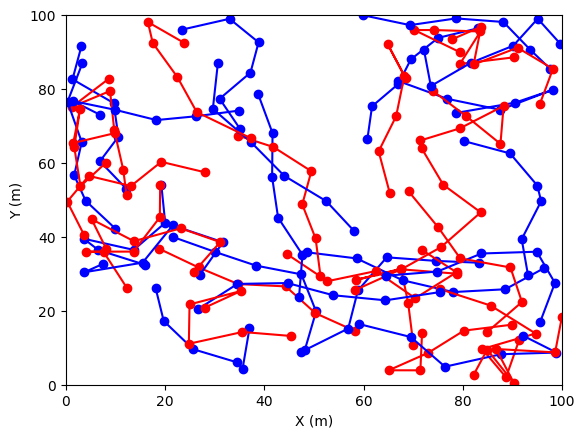
\includegraphics[height=2.4in,width=3.2in]{./Combined_path_illustration.png}
\caption{\label{fig:toyeg}
{\small Comparison of actual (red) and predicted (blue) locations.}}
\end{center}
\end{figure}


In Figure \ref{fig:toyeg}, we show the predicted and actual locations of all mobiles. As it can be seen, the actual locations
and the estimated locations are quite close. In the following, we present more
detailed analysis of the results.
% \begin{figure}[t]
% 	\begin{center}
% 	\subfigure[]{
% 	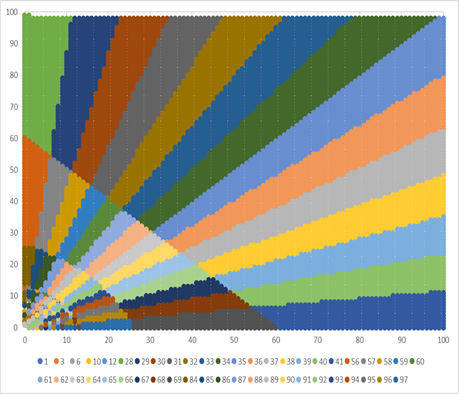
\includegraphics[height=2.5in, width=3.3in]{./Beam_map_LoS.png}
% 	%\caption{True Beam map for LoS}
% 	\label{fig:beam_map_cdf1}}
% 	\subfigure[]{
% 	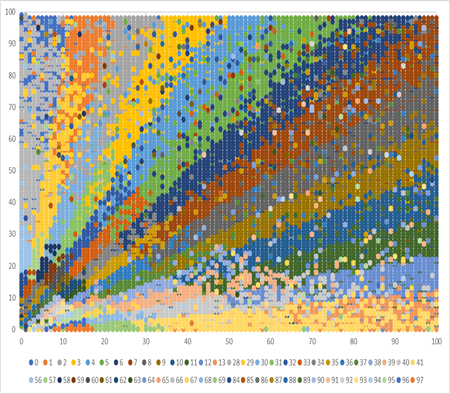
\includegraphics[height=2.5in, width=3.3in]{./Beam_map_MixedLoSNLoS.png}
% 	 %\caption{True Beam map for mixed LoS & NLoS}
% 	\label{fig:beam_map_cdf2}}
% 	\subfigure[]{
% 		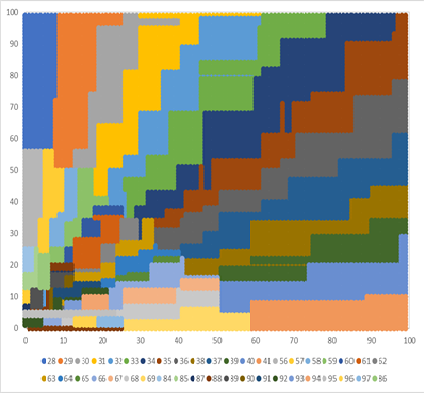
\includegraphics[height=2.5in, width=3.3in]{./Prediction_Beam_LoS.png}
% 	%	\caption{Predicted Beam map for LoS}
% 		\label{fig:beam_map_cdf3}}
% 		\subfigure[]{
% 	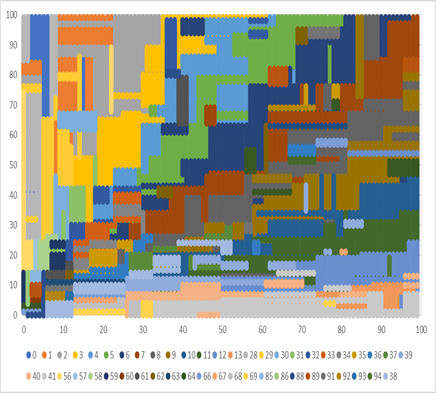
\includegraphics[height=2.5in, width=3.3in]{./Prediction_Beam_MixedLoSNLoS.png}
% 	%\caption{Predicted Beam map for NLoS}
% 	\label{fig:beam_map_cdf4}}
% 	\caption{Reported best beam indices distribution map \label{fig:leapperf} with different RF channel condition (LoS vs. MixedLoS\&NLoS)}
% 	\end{center}
% 	\end{figure}

\begin{figure}[t]
\begin{center}
 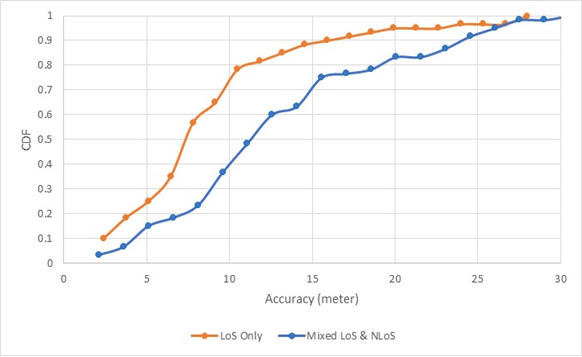
\includegraphics[height=2.5in, width=3.3in]{./Accuracy_ChannelModel.png}
\caption{CDF of accuracy.\label{fig:leapperf} with different RF channel condition (LoS vs. MixedLoS\&NLoS)}
\end{center}
\end{figure}
%{\em Inference accuarcy} 
% Figure~\ref{fig:beam_map_cdf1} and Figure~\ref{fig:beam_map_cdf2} illustrate the beam indices at different locations when RF channel conditons are LoS and mixed LoS\&NLoS, respectively. Figure~\ref{fig:beam_map_cdf3} and Figure~\ref{fig:beam_map_cdf4}
% shows the predicted beam indices using random forest classification. As we can see from these figures, when the training data is more spreaded as shown in Figure ~\ref{fig:beam_map_cdf2},
% the random forest classifier will divided the whole area into smaller region. The accuracy score \textbf{[QUESTION: should we define what accuracy score means? Is a value of 1 the best?]}  for LoS is 0.78 and for mixed LoS\&NLoS case is 0.57.

%{\em Accuracy CDF:} 
In Figure~\ref{fig:cdf1} and Figure~\ref{fig:cdf2}, we show the
accuracy distribution under two different type of RF channel condition, pure line of sight (LoS) and mixed LoS \& non-LoS(NLoS). More details of these scearions can be found in 
~\cite{3gpp38901}. With LoS channel, the median accuracy is around
$4m$, while with mixed LoS and NLoS channel, the median accuracy is around $12m$.These results have not included additional constraints such as users moving on prescribed paths such as walkways etc. as well as additional columns in the data matrix such as TA, etc. 
With this additional information, the localization accuracy is expected to improve further.

\section{Concluding Remarks}
\label{sec:concl}

In this paper, we have developed localization algorithms of mobile devices in 5G networks based on the measurement records 
We have shown median accuracy of 4m in LoS enviorment and 12m in mixed LoS and NLoS enviorments. 
when we incorporate the constraints of the 




%{
%\bibliography{community_bibliography}
%\bibliographystyle{unsrt}    
%}          

{%\scriptsize
\bibliographystyle{acm}
\bibliography{myref}
}


\end{document}


